%!TEX root = ../thesis.tex
%*******************************************************************************
%*********************************** Third Chapter *****************************
%*******************************************************************************

\chapter{Bioelectrical impedance plethysmography}  %Title of the First Chapter
\label{chapter impedance}

\ifpdf
    \graphicspath{{Chapter3/Figs/Raster/}{Chapter3/Figs/PDF/}{Chapter3/Figs/}}
\else
    \graphicspath{{Chapter3/Figs/Vector/}{Chapter3/Figs/}}
\fi

Before describing how impedance plethysmography operates, it is better to understand how the principle of bioelectrical impedance is defined. First of all, the term electrical impedance spectroscopy (EIS) is referred as the study of the absorption of energy depending upon the frequency of electromagnetic (EM) waves. When measurements are performed in a biological sample, then this method could be referred either as electrical impedance or bioelectrical impedance~\cite{ivorra2003bioimpedance}. The term to be used in this document will be bioelectrical electrical impedance. The EM spectrum is quite broad, and the interaction with tissue occurs in the frequency range from \SIrange[scientific-notation = engineering]{100}{10000000}{\hertz}~\cite{bertemes2002tissue}. In this thesis, the frequencies of interest are focused in the low-frequency range. Indeed, plethysmography devices operate commonly in the bandwidth below few \si{\kilo\hertz}.

The human body is constituted by four basic tissues known as epithelium which covers and protects the whole surface of the body, muscle which is in charge of the movement, connective tissue that supports and protect organs, and nervous tissue which provides the internal transmission line for the electrical impulses coming from the brain. Cells that constitute these tissues play a fundamental role in terms of current conduction when an analogue current (AC) is applied to the body~\cite{lvovich2012impedance}. Hence, impedance readings vary according to the parameters of these cells as well as its protein content. It is especially significant to understand the geometry and characteristics of the blood cells, which transport $0_2$ around the body. The functionality of these cells and amount per \si{\micro\litre} of human blood were described by table \ref{table:cell} in section \ref{section literature 1}.

As can be noticed from that table, RBC's statistically are more numerous than the other cells and it has particular resistive properties. Its disk shape can be ideally represented as a spherical particle with membranes around the surface, as represented by Figure \ref{fig:cell}. Live cells can be represented as multilayer cells where its internal cytoplasm has a characteristic permittivity ($\epsilon_{cp}$) and conductivity ($\rho_{cp}$). Likewise, these characteristics are similar to the one surrounding the cell called extracellular fluid ($\epsilon_m$ and $\rho_m$). However, the membrane has a very low permittivity ($\epsilon_{MBR}$) and conductivity ($\rho_{MBR}$) behaving as a dielectric. In contrast in dead cells the membrane becomes loose and does not provide resistance to electric current~\cite{lvovich2012impedance}.

\begin{figure}[!htpb]
	\centering
	\includegraphics[width=0.8\textwidth,keepaspectratio, trim={0cm 0cm 0cm 0cm},clip]{figure1}    
	\caption[Cell permeability and conductivity distribution]{Representation of a cell with its electric characteristics. Internal cytoplasm characteristic permittivity $\epsilon_{cp}$ and conductivity $\rho_{cp}$. Extracellular fluid permittivity $\epsilon_m$ and conductivity $\rho_m$). Membrane permittivity described as ($\epsilon_{MBR}$) and conductivity ($\rho_{MBR}$).}
	\label{fig:cell}
\end{figure}

A cell can change its internal cytoplasm by two different means either changing the permeability of their bilayer lipid membrane (BLM) or by using ionic channels or pumps. The BLM is about \SI{7}{\nano\meter} thick, by altering its permeability it allows lipids and water molecules to pass through~\cite{ivorra2003bioimpedance}. The interface extracellular-membrane-intracellular ($\rho_m \rightarrow \rho_{MBR} \leftarrow \rho_{cp}$) behaves as a capacitor because the membrane is a dielectric between two conductors, which is represented as $C_m$ in figure \ref{fig:cell model}.

On the other hand, parallel to BLM the ionic channels and pumps enhance membrane’s functionality. Ionic channels or “channel proteins” allow transport and exchange of certain types of ions such as $Na^{+}$, $K^{+}$, Chloride ($Cl^{-}$) and Calcium ($Ca^{2+}$) between the inside and outside of the cell~\cite{lvovich2012impedance}. Ion pumps are caused by sensitivity of the membrane to a voltage; it is also responsible for the membrane’s non–linear properties to low voltage. This pump also causes cell polarisation that allows the flow of ion charges in the body. Electrically, these channels act as a resistor ($R_m$).

\begin{figure*}[!htbp]
	\centering
	\begin{subfigure}[t]{0.5\textwidth}
		\centering
		\includegraphics[height=6.5cm]{figure2a}
		\caption{Cell's equivalent circuit model}
		\label{fig:cell model}
	\end{subfigure}%
	~ 
	\begin{subfigure}[t]{0.5\textwidth}
		\centering
		\includegraphics[height=6.5cm]{figure2b}
		\caption{Simplified circuit model}
		\label{fig:cell simp model}
	\end{subfigure}
	\caption[Electrical model of the cell]{Electrical model of the cell and its simplified version. $R_e$ is the resistivity of the extracellular medium, $R_i$ is the resistivity of the intracellular medium and $R_m$ and $C_m$ are the resistivity and capacitance of the membrane.}
	\label{fig:cell models}
\end{figure*}

According to previous analysis, the cell can be simplified in an equivalent electric circuit model as shown in Figure \ref{fig:cell models}. This model shows that if AC is pumped into the extracellular medium, there are two possible paths for the current to go through. One way is around the cell which is represented by the resistive characteristic of the extracellular medium ($R_e$). In the second route, current flows through the cell. Indeed, AC may flow initially either over the BLM which is a represented as a capacitance ($C_m$) or across ionic channels ($R_m$).Once in the cell, current travels via the intracellular medium ($R_i$) that is mostly resistive. Lastly, the electrical current leaves the cell through the membrane, which it is again the same $C_m$ and $R_m$.

Since $C_m$ and $R_m$ have the same values when the current enters and exits the cell, this can be simplified in the electric model as two resistors in series ($2R_m$) and two capacitances in parallel ($C_m/2$) as can be seen in figure \ref{fig:cell simp model}.


When an EM field is applied to the tissue, cells respond according to the frequency applied showing three distinctive areas in the spectrum as described by Schawn et al.~\cite{schwan1957electrical,schwan1962electrical}. Figure \ref{fig:ABG dispersion} displays the dielectric response against frequency, which reveals valuable information about the functional and structural properties of the cell~\cite{lvovich2012impedance}. According to the graph, there are three denominating areas $\alpha$, $\beta$ and $\gamma$ dispersion. Firstly, $\alpha$ dispersion (from \SI{10}{\hertz} to a few \si{\kilo\hertz}) is generally associated with frequency dependent properties of the cells’ membrane. Secondly, $\beta$ dispersion (\SI{10}{\kilo\hertz} to several \si{\mega\hertz}) is related to the dielectric property of the cell membrane and the interaction between the internal and external mediums. Finally, $\gamma$ dispersion (> \SI{10}{\giga\hertz}) is due to dielectric relaxation of bulk dispersing media, the Debye dispersion in water (\SI{17}{\giga\hertz}) and the presence of small molecules. 

\begin{figure}[!htpb]
	\centering
	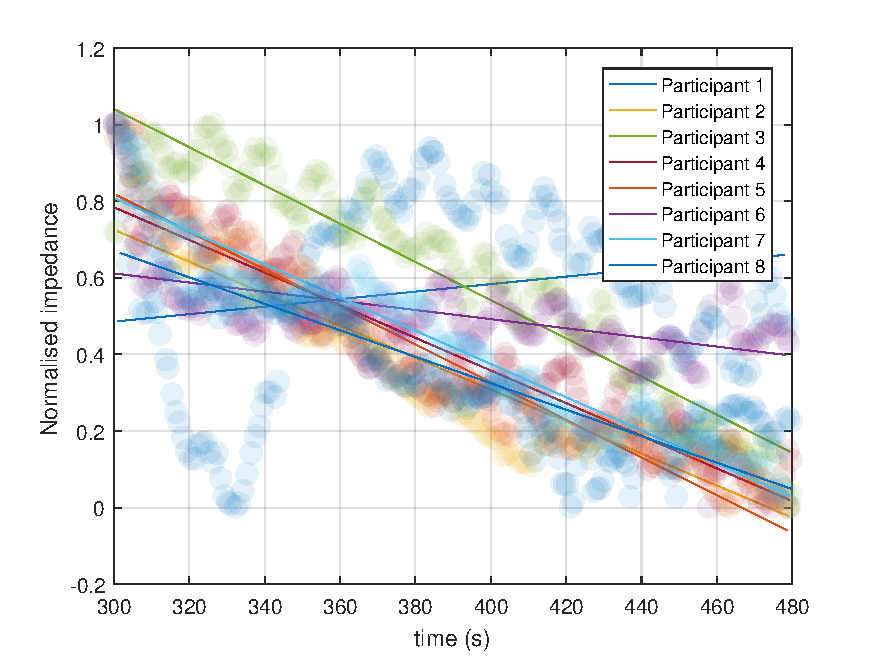
\includegraphics[width=0.8\textwidth,keepaspectratio, trim={0cm 1cm 0cm 0cm},clip]{figure3}    
	\caption[Alpha, Bet y Gama dispersion]{Representation of a cell with its electric characteristics. Internal cytoplasm characteristic permittivity $\epsilon_{cp}$ and conductivity $\rho_{cp}$. Extracellular fluid permittivity $\epsilon_m$ and conductivity $\rho_m$). Membrane permittivity described as ($\epsilon_{MBR}$) and conductivity ($\rho_{MBR}$).}
	\label{fig:ABG dispersion}
\end{figure}

In addition, the $\beta$ dispersion region provides supplementary information about the cell. Lvovich \cite{lvovich2012impedance} has divided this area into three subregions depending on the interaction of the electrical current with the cell. The $\beta_1$ relaxation is due to the capacitive membrane $C_m$, occurring in the low \si{\kilo\hertz} range. When the frequency is increased between \si{\kilo\hertz} and low \si{\mega\hertz} range the internal cytoplasm of the cell can produce a $\beta_3$ dispersion because of a change from resistive to capacitive conduction. However, this capacitive component is often disregarded simplifying the model into just a resistive element $R_i$. Ultimately, $\beta_2$ happens in the range of low \si{\mega\hertz} when the electrical charge movement through the cell shifts to a capacitive conduction.

This research document is centred in the $\beta$ dispersion region between \SIrange[scientific-notation = engineering]{100}{1000000}{\hertz}. The impedance plethysmography device designed described in chapter \ref{chapter design} is capable to operate within this bandwidth. 

The ideal electrical model of the cell shown in figure \ref{fig:cell models} is a very close approximation that allows predicting bioelectrical impedance behaviour for dilute cell suspension. However, tissue is more complex than this having extra components to be analysed. For instance, tissue like muscle exhibits extreme anisotropy (conductivity is not the same when measured in different directions) \cite{lvovich2012impedance,dean2008electrical,foster1995dielectric}. Therefore, the position where electrodes are placed influences in the impedance of the readings. Also the change of volume of the blood vessels during the heart’s systole and diastole also changes impedance magnitude readings which is the principle used by impedance plethysmography. 

Another example of this is in the myocardial muscle studied in pigs where two superimposed depressions were observed in-between \SIrange[scientific-notation = engineering]{10}{1000000}{\hertz} ~\cite{casas1999vivo}. Different resistivity values have been obtained when measuring bioelectrical impedance during the cardiac cycle longitudinally and transversally \cite{steendijk1993four}. \mynote{Maybe this paragraph is not requires as might refer to death cells rather than plethysmography}

%********************************** %First Section  **************************************
\section{Impedance plethysmography principle} %Section - 1.1 
\label{section impedance 1}

As previously described in section \ref{section literature 3.5}, iPG is the measurement of volume changes through the equivalent bioelectrical impedance of a part of the human body~\cite{corciova2011peripheral}. In this document is presented the measurements from an in-vivo studio of the plethysmographic changes in a segment of the left forearm. As it can be deduced, one would assume that this segment of the upper limb could be modelled as a cylinder within a cylinder. Where the inner cylinder represents a blood vessel and the outermost is the surrounding tissue. 

For mathematical analysis, a single cylinder will be initially studied and then the double cylinder model. An ideal circular solid model can be applied where the cross-sectional area might have a circular or elliptical form. Hence, measurement of electrical impedance might depend on its geometry. The following equation illustrates the segment’s geometry effects either conductance ($G$) or resistance ($R$). However, this document will use the resistance equivalent during the mathematical explanation.

\begin{align}
\label{eq:resistivity}
R=\sigma\frac{L}{A}
\end{align}




%********************************** %Second Section  *************************************
\section{Why do we use loren ipsum?} %Section - 1.2


%********************************** % Third Section  *************************************
\section{Where does it come from?}  %Section - 1.3 
\label{section1.3}

%********************************** %Nomenclatures in chapter  **************************************
\nomenclature[z-EM]{EM}{Electromagnetic}
\nomenclature[z-EIS]{EIS}{Electrical impedance spectroscopy}
\nomenclature[z-BLM]{BLM}{Bilayer lipid membrane}